\begin{figure}[H]
\centering
\resizebox{0.45\textwidth}{!}
{
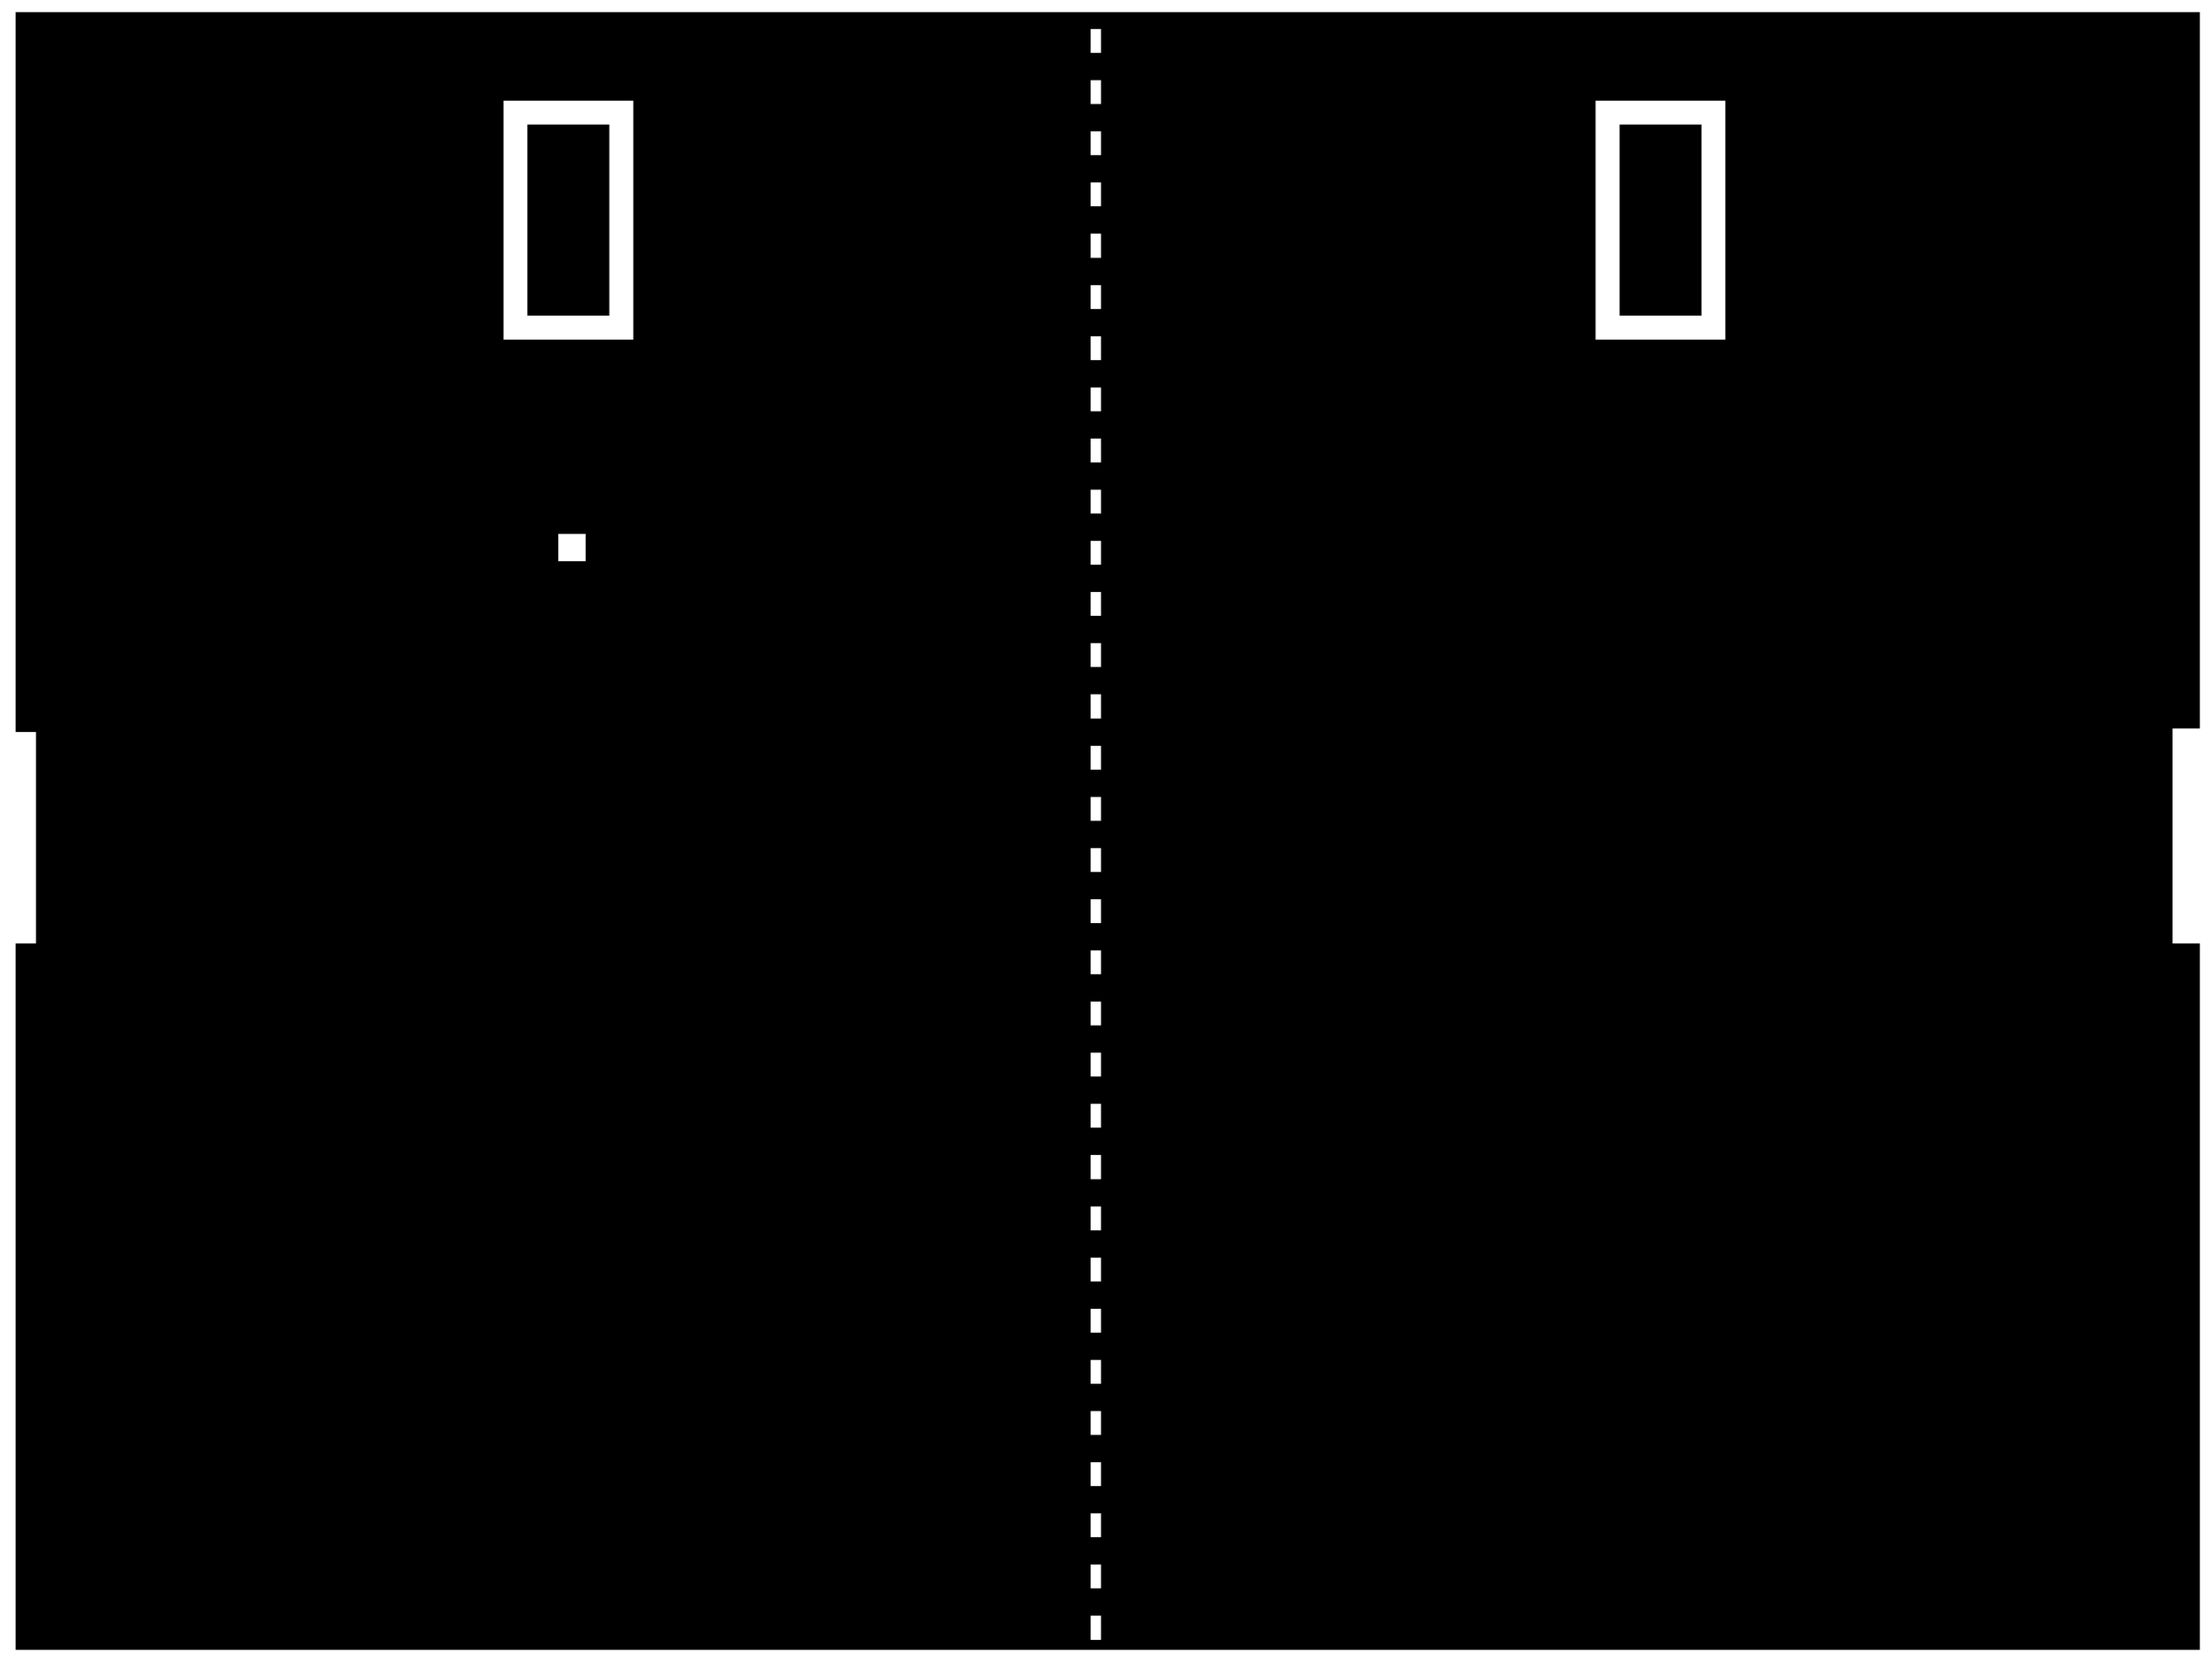
\begin{tikzpicture}[x = 1mm, y = 1mm]
    
    \def\width  {640}
    \def\height {480}

    % screen
    \path [fill = black] (1, 1) rectangle ++(\width, \height);
    % paddle 1
    \path [fill = white] (1 - 1, \height / 2 - 32) rectangle ++(8 - 1, 63 - 1);
    % paddle 2
    \path [fill = white] (\width - 8 + 1, \height / 2 - 32) rectangle ++(8, 63);
    % ball
    \path [fill = white] (160, 320) rectangle ++(8, 8);
    % Number 1
    \path [fill = white] (\width / 4 - 16, \height - 32) 
        rectangle ++(32 - 1,   8 - 1)
        rectangle ++(8 - 1,  -64 + 1)
        rectangle ++(-32 + 1, -8 + 1)
        rectangle ++(-8 + 1,  64 - 1);
    % Number 2
    \path [fill = white] (3 * \width / 4 - 16, \height - 32) 
        rectangle ++(32 - 1,   8 - 1)
        rectangle ++(8 - 1,  -64 + 1)
        rectangle ++(-32 + 1, -8 + 1)
        rectangle ++(-8 + 1,  64 - 1);
        
    % middle line
    \foreach \i in {1, 16, ..., \height}
         \path [fill = white] (\width / 2 - 4, \i + 3) rectangle ++(4 - 1, 8 - 1);

\end{tikzpicture}
}
\caption{Janela do jogo}
\label{fig:game_screen}
\end{figure}